\documentclass[nofonts,]{tufte-handout}

% ams
\usepackage{amssymb,amsmath}

\usepackage{ifxetex,ifluatex}
\usepackage{fixltx2e} % provides \textsubscript
\ifnum 0\ifxetex 1\fi\ifluatex 1\fi=0 % if pdftex
  \usepackage[T1]{fontenc}
  \usepackage[utf8]{inputenc}
\else % if luatex or xelatex
  \makeatletter
  \@ifpackageloaded{fontspec}{}{\usepackage{fontspec}}
  \makeatother
  \defaultfontfeatures{Ligatures=TeX,Scale=MatchLowercase}
  \makeatletter
  \@ifpackageloaded{soul}{
     \renewcommand\allcapsspacing[1]{{\addfontfeature{LetterSpace=15}#1}}
     \renewcommand\smallcapsspacing[1]{{\addfontfeature{LetterSpace=10}#1}}
   }{}
  \makeatother
\fi

% graphix
\usepackage{graphicx}
\setkeys{Gin}{width=\linewidth,totalheight=\textheight,keepaspectratio}

% booktabs
\usepackage{booktabs}

% url
\usepackage{url}

% hyperref
\usepackage{hyperref}

% units.
\usepackage{units}


\setcounter{secnumdepth}{-1}

% citations
\usepackage{natbib}
\bibliographystyle{plainnat}

%% tint override
\setcitestyle{round} 

% pandoc syntax highlighting

% longtable
\usepackage{longtable,booktabs}

% multiplecol
\usepackage{multicol}

% strikeout
\usepackage[normalem]{ulem}

% morefloats
\usepackage{morefloats}


% tightlist macro required by pandoc >= 1.14
\providecommand{\tightlist}{%
  \setlength{\itemsep}{0pt}\setlength{\parskip}{0pt}}

% title / author / date
\title{Gene cloning and Recombinant DNA technology}
\author{Deependra Dhakal}
\date{2019-06-15}

%% -- tint overrides
%% fonts, using roboto (condensed) as default
\usepackage[sfdefault,condensed]{roboto}
%% also nice: \usepackage[default]{lato}

%% colored links, setting 'borrowed' from RJournal.sty with 'Thanks, Achim!'
\RequirePackage{color}
\definecolor{link}{rgb}{0.1,0.1,0.8} %% blue with some grey
\hypersetup{
  colorlinks,%
  citecolor=link,%
  filecolor=link,%
  linkcolor=link,%
  urlcolor=link
}

%% macros
\makeatletter

%% -- tint does not use italics or allcaps in title
\renewcommand{\maketitle}{%     
  \newpage
  \global\@topnum\z@% prevent floats from being placed at the top of the page
  \begingroup
    \setlength{\parindent}{0pt}%
    \setlength{\parskip}{4pt}%
    \let\@@title\@empty
    \let\@@author\@empty
    \let\@@date\@empty
    \ifthenelse{\boolean{@tufte@sfsidenotes}}{%
      %\gdef\@@title{\sffamily\LARGE\allcaps{\@title}\par}%
      %\gdef\@@author{\sffamily\Large\allcaps{\@author}\par}%
      %\gdef\@@date{\sffamily\Large\allcaps{\@date}\par}%
      \gdef\@@title{\begingroup\fontseries{b}\selectfont\LARGE{\@title}\par}%
      \gdef\@@author{\begingroup\fontseries{l}\selectfont\Large{\@author}\par}%
      \gdef\@@date{\begingroup\fontseries{l}\selectfont\Large{\@date}\par}%
    }{%
      %\gdef\@@title{\LARGE\itshape\@title\par}%
      %\gdef\@@author{\Large\itshape\@author\par}%
      %\gdef\@@date{\Large\itshape\@date\par}%
      \gdef\@@title{\begingroup\fontseries{b}\selectfont\LARGE\@title\par\endgroup}%
      \gdef\@@author{\begingroup\fontseries{l}\selectfont\Large\@author\par\endgroup}%
      \gdef\@@date{\begingroup\fontseries{l}\selectfont\Large\@date\par\endgroup}%
    }%
    \@@title
    \@@author
    \@@date
  \endgroup
  \thispagestyle{plain}% suppress the running head
  \tuftebreak% add some space before the text begins
  \@afterindentfalse\@afterheading% suppress indentation of the next paragraph
}

%% -- tint does not use italics or allcaps in section/subsection/paragraph
\titleformat{\section}%
  [hang]% shape
  %{\normalfont\Large\itshape}% format applied to label+text
  {\fontseries{b}\selectfont\Large}% format applied to label+text
  {\thesection}% label
  {1em}% horizontal separation between label and title body
  {}% before the title body
  []% after the title body

\titleformat{\subsection}%
  [hang]% shape
  %{\normalfont\large\itshape}% format applied to label+text
  {\fontseries{m}\selectfont\large}% format applied to label+text
  {\thesubsection}% label
  {1em}% horizontal separation between label and title body
  {}% before the title body
  []% after the title body

\titleformat{\paragraph}%
  [runin]% shape
  %{\normalfont\itshape}% format applied to label+text
  {\fontseries{l}\selectfont}% format applied to label+text
  {\theparagraph}% label
  {1em}% horizontal separation between label and title body
  {}% before the title body
  []% after the title body

%% -- tint does not use italics here either
% Formatting for main TOC (printed in front matter)
% {section} [left] {above} {before w/label} {before w/o label} {filler + page} [after]
\ifthenelse{\boolean{@tufte@toc}}{%
  \titlecontents{part}% FIXME
    [0em] % distance from left margin
    %{\vspace{1.5\baselineskip}\begin{fullwidth}\LARGE\rmfamily\itshape} % above (global formatting of entry)
    {\vspace{1.5\baselineskip}\begin{fullwidth}\fontseries{m}\selectfont\LARGE} % above (global formatting of entry)
    {\contentslabel{2em}} % before w/label (label = ``II'')
    {} % before w/o label
    {\rmfamily\upshape\qquad\thecontentspage} % filler + page (leaders and page num)
    [\end{fullwidth}] % after
  \titlecontents{chapter}%
    [0em] % distance from left margin
    %{\vspace{1.5\baselineskip}\begin{fullwidth}\LARGE\rmfamily\itshape} % above (global formatting of entry)
    {\vspace{1.5\baselineskip}\begin{fullwidth}\fontseries{m}\selectfont\LARGE} % above (global formatting of entry)
    {\hspace*{0em}\contentslabel{2em}} % before w/label (label = ``2'')
    {\hspace*{0em}} % before w/o label
    %{\rmfamily\upshape\qquad\thecontentspage} % filler + page (leaders and page num)
    {\upshape\qquad\thecontentspage} % filler + page (leaders and page num)
    [\end{fullwidth}] % after
  \titlecontents{section}% FIXME
    [0em] % distance from left margin
    %{\vspace{0\baselineskip}\begin{fullwidth}\Large\rmfamily\itshape} % above (global formatting of entry)
    {\vspace{0\baselineskip}\begin{fullwidth}\fontseries{m}\selectfont\Large} % above (global formatting of entry)
    {\hspace*{2em}\contentslabel{2em}} % before w/label (label = ``2.6'')
    {\hspace*{2em}} % before w/o label
    %{\rmfamily\upshape\qquad\thecontentspage} % filler + page (leaders and page num)
    {\upshape\qquad\thecontentspage} % filler + page (leaders and page num)
    [\end{fullwidth}] % after
  \titlecontents{subsection}% FIXME
    [0em] % distance from left margin
    %{\vspace{0\baselineskip}\begin{fullwidth}\large\rmfamily\itshape} % above (global formatting of entry)
    {\vspace{0\baselineskip}\begin{fullwidth}\fontseries{m}\selectfont\large} % above (global formatting of entry)
    {\hspace*{4em}\contentslabel{4em}} % before w/label (label = ``2.6.1'')
    {\hspace*{4em}} % before w/o label
    %{\rmfamily\upshape\qquad\thecontentspage} % filler + page (leaders and page num)
    {\upshape\qquad\thecontentspage} % filler + page (leaders and page num)
    [\end{fullwidth}] % after
  \titlecontents{paragraph}% FIXME
    [0em] % distance from left margin
    %{\vspace{0\baselineskip}\begin{fullwidth}\normalsize\rmfamily\itshape} % above (global formatting of entry)
    {\vspace{0\baselineskip}\begin{fullwidth}\fontseries{m}\selectfont\normalsize\rmfamily} % above (global formatting of entry)
    {\hspace*{6em}\contentslabel{2em}} % before w/label (label = ``2.6.0.0.1'')
    {\hspace*{6em}} % before w/o label
    %{\rmfamily\upshape\qquad\thecontentspage} % filler + page (leaders and page num)
    {\upshape\qquad\thecontentspage} % filler + page (leaders and page num)
    [\end{fullwidth}] % after
}{}

  
\makeatother


\usepackage{booktabs}
\usepackage{longtable}
\usepackage{array}
\usepackage{multirow}
\usepackage{wrapfig}
\usepackage{float}
\usepackage{colortbl}
\usepackage{pdflscape}
\usepackage{tabu}
\usepackage{threeparttable}
\usepackage{threeparttablex}
\usepackage[normalem]{ulem}
\usepackage{makecell}
\usepackage{xcolor}

\begin{document}

\maketitle




\clearpage

\hypertarget{recombinant-dna-technology}{%
\section{Recombinant DNA technology}\label{recombinant-dna-technology}}

In 1972, two researchers met at a conference in Hawaii to discuss
plasmids, the small rings of extrachromosomal DNA found in bacteria.
Herbert W. Boyer, PhD, was a faculty member at the University of
California, San Diego, and he was studying restriction and modification
enzymes. He had just presented his research on EcoRI. Stanley N. Cohen,
MD, was a faculty member at Stanford, and he was interested in how
plasmids could confer resistance to different antibiotics. His lab
perfected laboratory transformation of Escherichia coli using calcium
chloride to permeabilize the cells. After the talks ended, the two met
over corned beef sandwiches and combined their two ideas.

\begin{figure*}
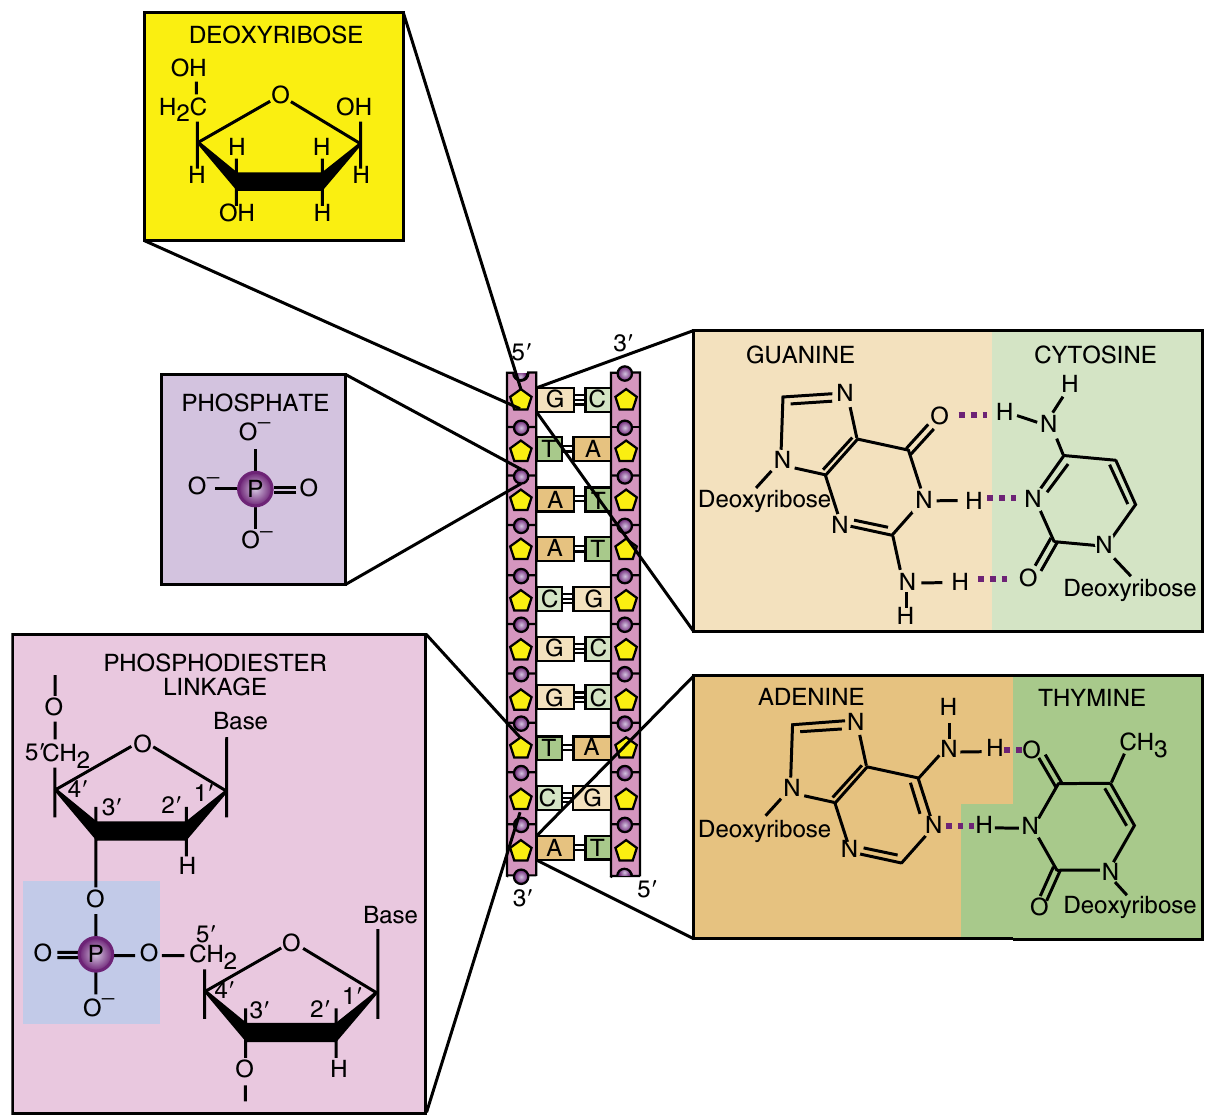
\includegraphics[width=0.7\linewidth]{./images/dna_structure_a} \caption[DNA has two strands antiparallel to each other]{DNA has two strands antiparallel to each other. The structure of the subcomponents is shown to the sides.}\label{fig:nucleic-acid}
\end{figure*}
\begin{figure*}
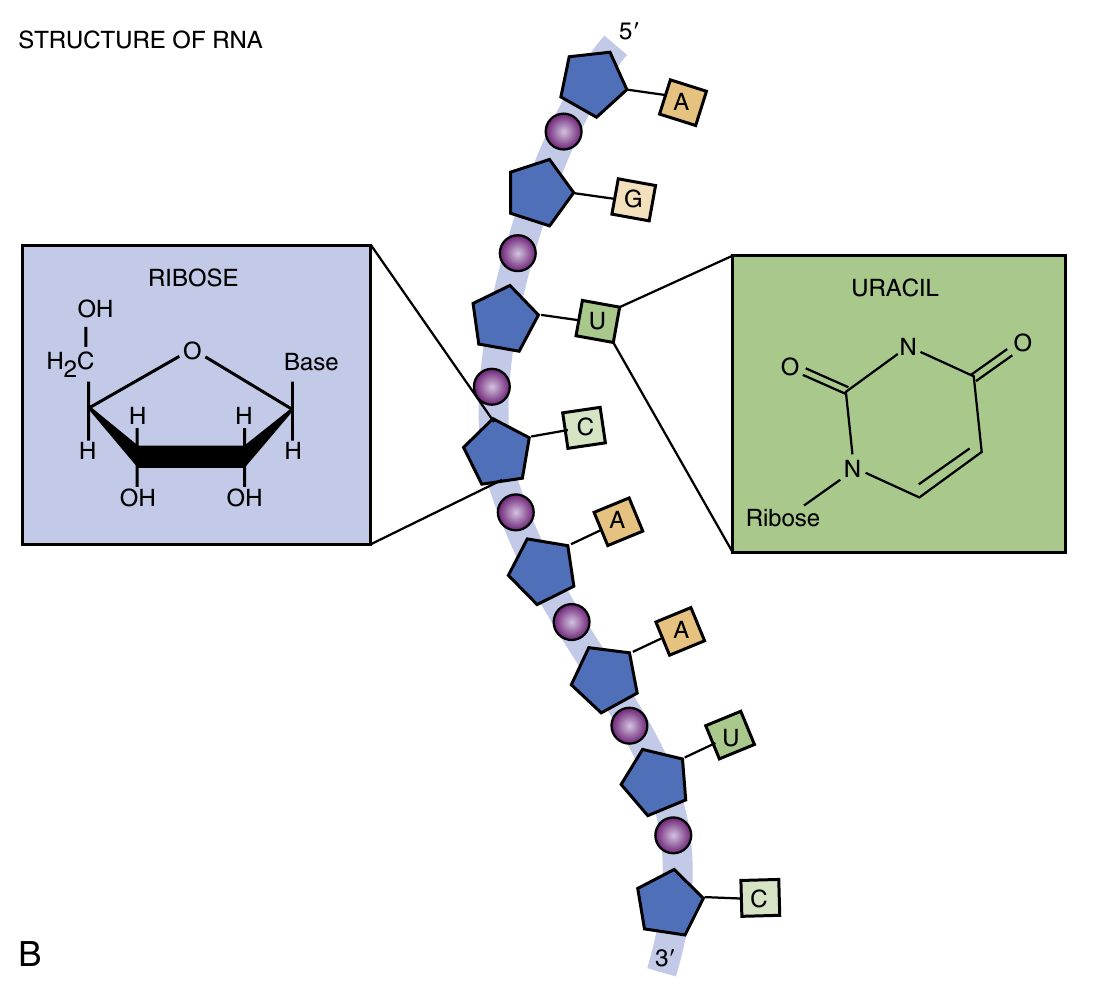
\includegraphics[width=0.7\linewidth]{./images/dna_structure_b} \caption[RNA is usually single-stranded and has two chemical differences from DNA]{RNA is usually single-stranded and has two chemical differences from DNA. First, an extra hydroxyl group (-OH) is found at the 2 prime position of ribose, and second, thymine is replaced by uracil.}\label{fig:nucleic-acid}
\end{figure*}

They isolated different fragments of DNA from animals, other bacteria,
and viruses and, using restriction enzymes, ligated the fragments into a
small plasmid from E. coli. This was the first recombinant DNA made.
Finally, they transformed the engineered plasmid back into E. coli. The
cells expressed the normal plasmid genes as well as those inserted into
the plasmid artificially. This sparked the revolution in genetic
engineering, and since then every biotechnology lab has used some
variation of their technique. Boyer and Cohen applied for a patent on
recombinant DNA technology. In fact, Boyer cofounded Genentech with
Robert Swanson, a venture capitalist. Genentech is one of the first
biotechnology companies in the United States, and under Boyer and
Swanson, the company produced human somatostatin in E. coli.

\hypertarget{dna-isolation-and-purification}{%
\subsection{DNA Isolation and
Purification}\label{dna-isolation-and-purification}}

Isolating DNA from different organism is the basic to all biotechnology
research. Bacteria, having little structure beyond the cell wall and
cell membrane, are the easiest to manipulate.

Considering two distinct forms of DNA: The nuclear/genomic DNA and the
plasmid DNA, distinction between these two is made based on their sizes.
Following steps are necessary to release the DNA from a cell:

\begin{enumerate}
\def\labelenumi{\arabic{enumi}.}
\tightlist
\item
  Destruction of cell membrane. (Lysozyme digestion of peptidoglycan in
  bacteria)
\item
  Bursting of cell membrane by destruction of lipid bilayer (by
  detergent such as sodium dodecyl sulfate (SDS)). In plants and
  animals, tissue samples are generally ground up to release the
  intracellular components.
\item
  Separation of intracellular components from the insoluble remains
  (cellular membranes, bones, cartilage, etc.) by either centrifugation
  or chemical extraction.
\item
  Extraction of unwanted proteins from DNA with phenol (Dissolves
  60\%-70\% of all living matter).
\end{enumerate}

Two phases are formed, one that of proteins dissolved in phenol and the
other of nucleic acids in the aqueous layer. The two phases are
separated by centrifugation, and the aqueous DNA layer is removed form
the phenol.

The sample still contains RNA along with the DNA. The enzyme rbonuclease
(RNase) digests RNA into small ribonucleotide fragments. Treating this
solution with alcohol leaves extremely large DNA fall out of the aqueous
phase, while ribonucleotides stay soluble, thus favoring centrifugation
extraction of DNA.

\hypertarget{electrophoresis-separates-dna-fragments-by-size}{%
\subsection{Electrophoresis separates DNA fragments by
size}\label{electrophoresis-separates-dna-fragments-by-size}}

Gel electrophoresis is used to separate DNA fragments by size. The gel
consists of agarose, a polysaccharide extracted from seaweed that
behaves like gelatin. Agarose is available in powdered form
commercially.

For visualizing DNA agarose gel is solidified, after subsequent cooling
once the powder-water mixture is heated, into a rectangular slab about
1/4 inch thick by casting the molten liquid into a special tray. To make
small wells or holes at one end of the gel, comb is inserted before the
gel hardens.

Gel electrophoresis uses electric current to separate DNA molecules by
size. The agarose slab is immersed in a buffer-filled tank that has a
positive electrode at one end and a negative electrode at the other. DNA
samples are loaded into the wells, and when an electrical field is
applied, the DNA migrates through the gel. The phosphate backbone of DNA
is negatively charged, so it moves away from the negative electrode and
toward the positive electrode. Polymerized agarose acts as a sieve with
small holes between the tangled chains of agarose. The DNA must migrate
through these gaps. Agarose separates the DNA by size because larger
pieces of DNA are slowed down more by the agarose.

To visualize the DNA, the agarose gel is removed from the tank and
immersed into a solution of ethidium bromide. This dye intercalates
between the bases of DNA or RNA, although less dye binds to RNA because
it is single-stranded. When the gel is exposed to ultraviolet light, it
fluoresces bright orange. Since ethidium bromide is a mutagen and
carcinogen, less dangerous DNA dyes such as SYBR Safe (R) are used in
most laboratories now. In Figure \ref{fig:gel-electrophoresis}, the DNA
fragments are visualized by a positively charged dye from the thiazin
family. The dye interacts with the negatively charged backbone of the
DNA and is a nontoxic alternative that does not require ultraviolet
light sources.

Important point to note is that, size of DNA being examined affects what
type of gel is used. Size of DNA molecules can be determined by
comparing to a set of molecular weight standards run in a different
well. Because the standards are of known size, the experimental DNA
fragment can be compared directly.

In agarose gel, DNA fragments from 200 to 10000 bp can be separated. For
DNA fragments of 50-1000 bp differences, polyacrylamide gels are used
instead. These gels are able to resolve DNA fragments by only one base
pair and are essential to sequencing of DNA with Sanger method. For very
large fragments (10 kbp to 10 mbp), agarose gel is used, but the current
is alternated at two different angles.

\begin{figure}
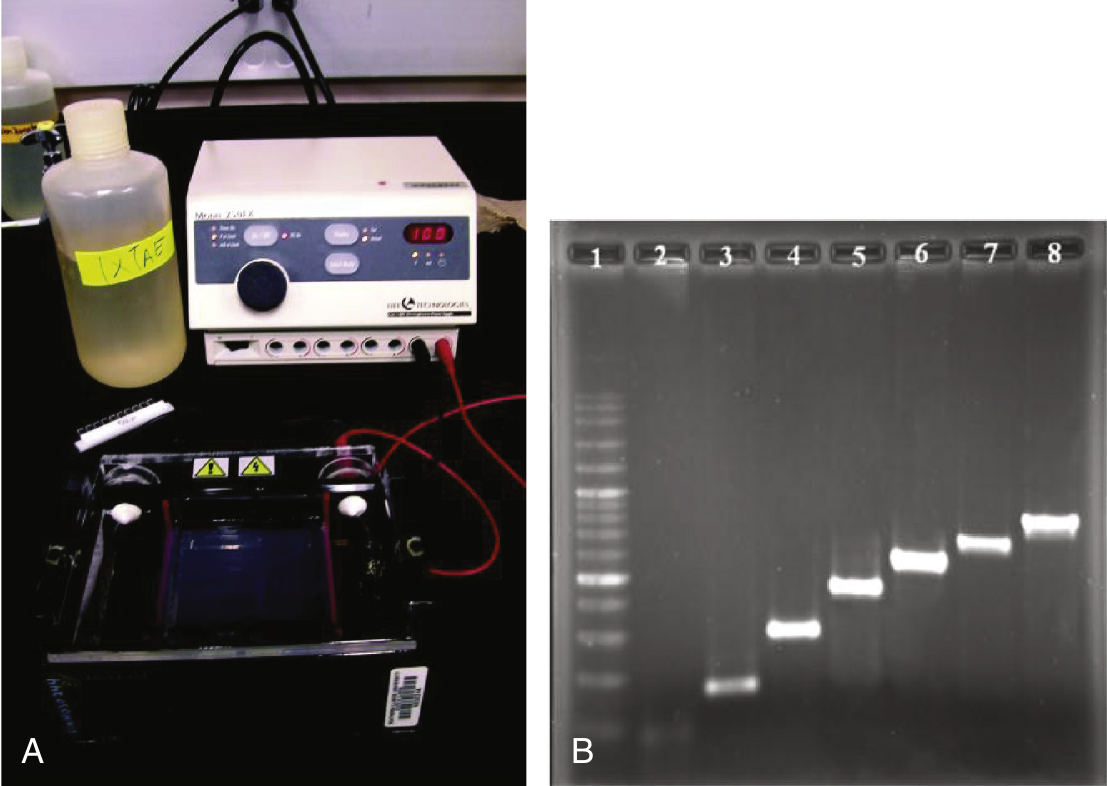
\includegraphics[width=0.95\linewidth]{./images/electrophoresis} \caption[(A) Photo of electrophoresis supplies]{(A) Photo of electrophoresis supplies. Electrophoresis chamber holds an agarose gel in the center portion, and the rest of the tank is filled with buffer solution. The red and black leads are then attached to an electrical source. FisherBiotech Horizontal Electrophoresis Systems, Midigel System; Standard; 13 $\times$ 16-cm gel size; 800 mL buffer volume; Model No. FB-SB-1316. (B) Agarose gel separation of DNA. The size of the fragments can be calculated by comparing them to the standard DNA marker in lane 1. The brighter bands in the marker are 1000 base pairs and 500 base pairs, with the 1000 base-pair marker closer to the wells (marked with numbers 1–8).}\label{fig:gel-electrophoresis}
\end{figure}

\marginnote{Fragments of DNA are separated by size using gel electrophoresis. A current causes the DNA fragments to move away from the negative electrode and toward the positive. As the DNA travels through agarose, the larger fragments get stuck in the gel pores more than the smaller DNA fragments.
 Pulsed field gel electrophoresis separates large pieces of DNA by alternating the electric current at right angles.}

\hypertarget{restriction-enzymes-cut-dna-ligase-joins-dna}{%
\subsection{Restriction enzymes cut DNA; Ligase joins
DNA}\label{restriction-enzymes-cut-dna-ligase-joins-dna}}

In practice entire set of nuclear DNA is not of particular interest in
visualization, after isolation and separation. DNA should be cut to
fragments of different sizes. Naturally occuring \emph{restriction
enzymes} or \emph{restriction endonucleases} come into rescue in this
operation. These bacterial enzymes bind to specific recognition sites on
DNA and cut the backbone of both strands. They evolved to protect
bacteria from foreign DNA, such as viruses. The enzymes do not cut their
own cell's DNA because they are \emph{methylation} sensitive. Bacteria
produce \emph{modification enzymes} that recognize the same sequence as
the corresponding restriction enzyme. These methylate each recognition
site in the bacterial genome.

\begin{marginfigure}
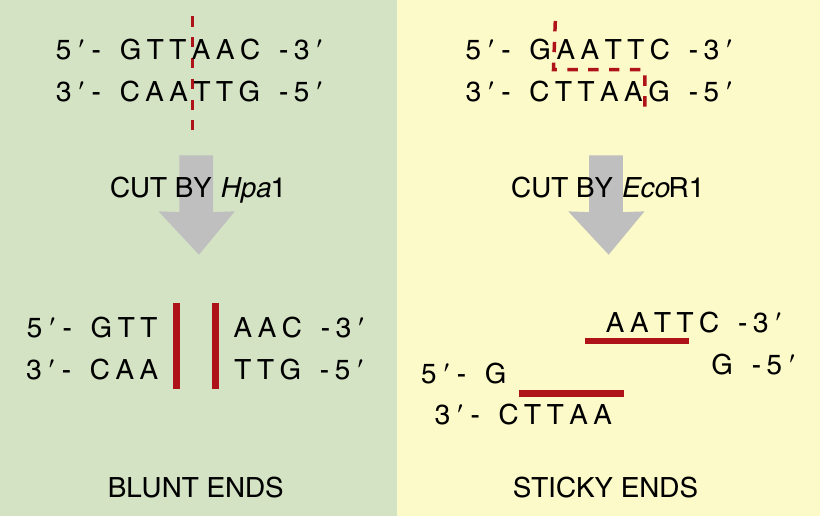
\includegraphics[width=0.95\linewidth]{./images/restriction_enzymes} \caption{\textbf{Type II Restriction Enzymes -- Blunt versus Sticky ends} \newline \textit{Hpal} is a bunt-end restriction enzyme; that is, it cuts both strands of DNA in exactly the same position.  extit{EcoR}I is a sticky-end restriction enzyme. The enzyme cuts between the G and A on both strands, which generates four base-pair overhangs on the ends of the DNA. Since these ends may base pair with complementary sequences, they are considered 'sticky'.}\label{fig:restriction-enzymes}
\end{marginfigure}

Restriction enzymes have been exploited to cut DNA at specific sites,
since each restriction enzyme has a particular recognition sequence.
Difference in cleavage site determine the type of restriction enzyme.

\begin{itemize}
\tightlist
\item
  Type I restriction enzymes cut the DNA strand 1000 or more base pairs
  from the recognition sequence.
\item
  Type II restriction enzymes cut in the middle of the recognition
  sequence and are the most useful in genetic engineering. The Type II
  restriction enzymes can form \emph{both} sticky or \emph{blunt} ends.
\end{itemize}

The recognition sequences of Type II restriction enzymes are usually
inverted repeats so that the enzymes cut between the same bases on the
both strands.

\begin{figure}
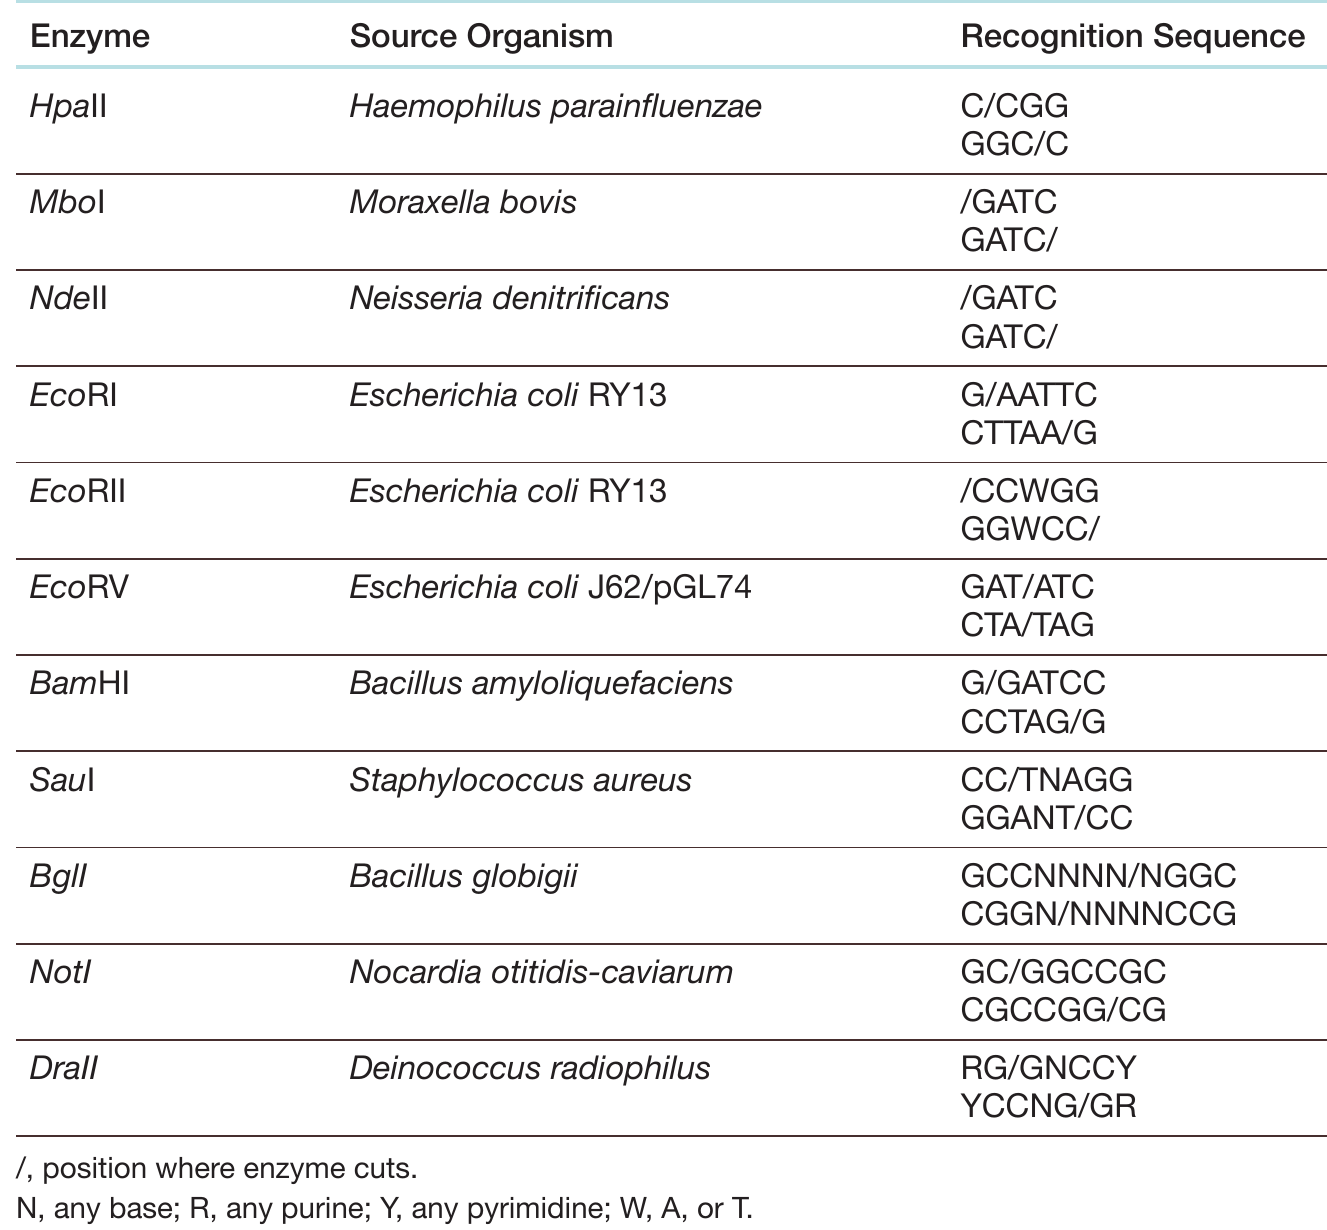
\includegraphics[width=0.9\linewidth]{./images/restriction_enzymes_ex} \caption[Common restriction enzymes]{Common restriction enzymes}\label{fig:restriction-enzymes-ex}
\end{figure}

The number of base pairs in the recognition sequence determines the
likelihood of cutting. So to generate fewer, longer fragments,
restriction enzymes with siz or more base-pair recognition sequences are
used. Conversely, four base-pair enzymes give more, shorter fragments
from the same original segment of DNA.

\begin{marginfigure}
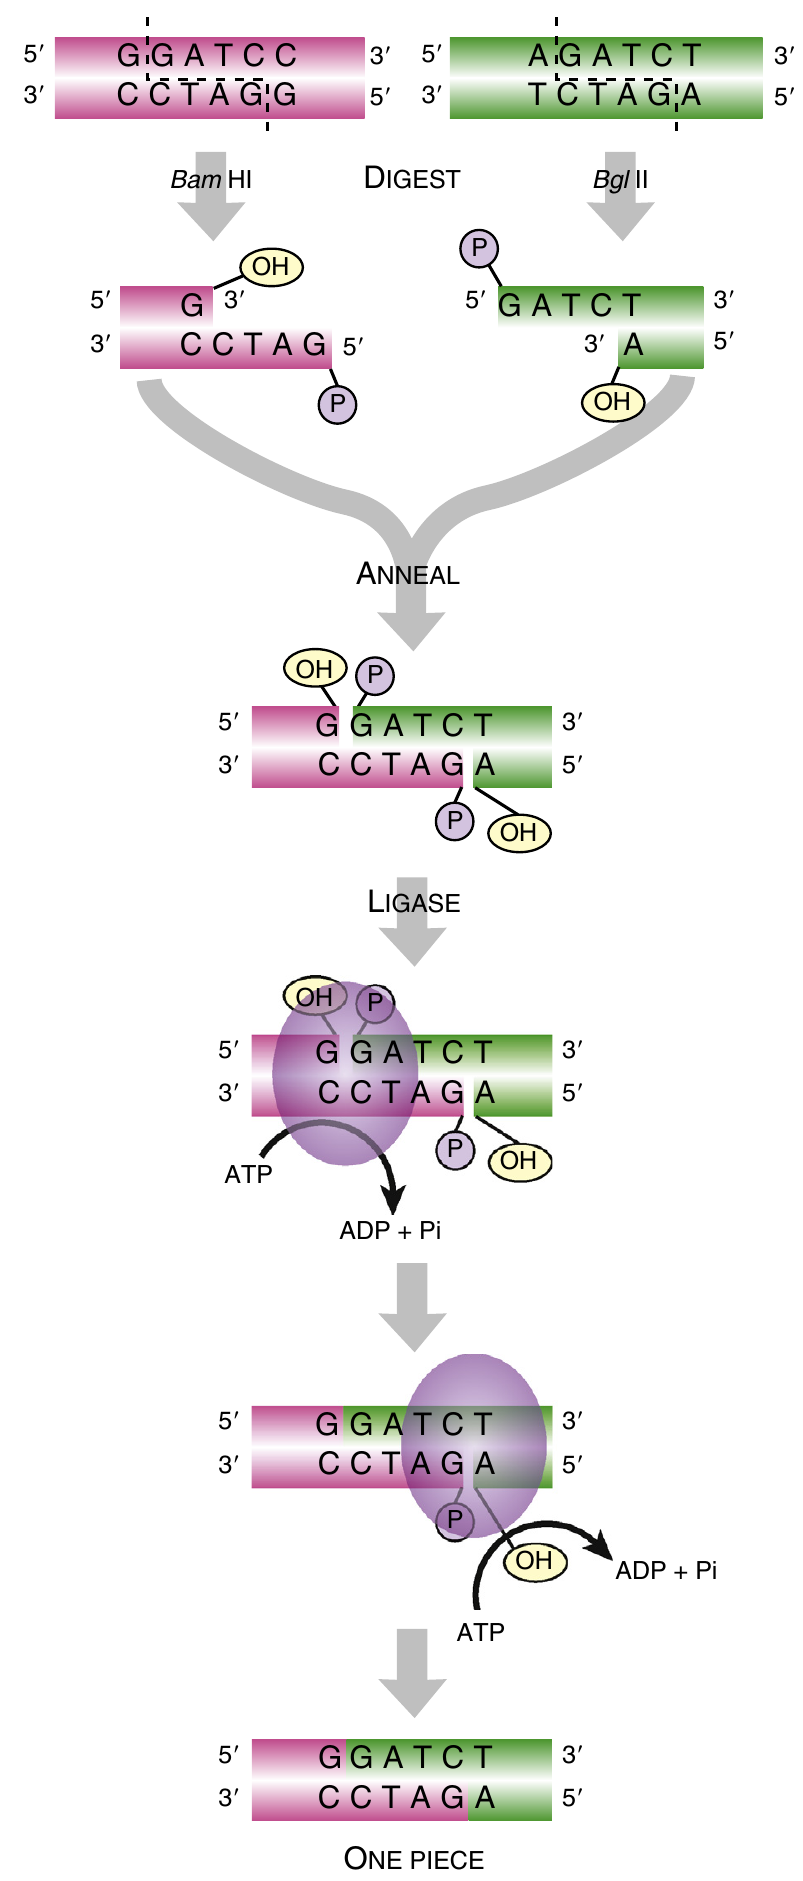
\includegraphics[width=0.95\linewidth]{./images/restriction_ligation} \caption[\textbf{Compatible overhangs are linked using DNA Ligase}\newline BamHI and Bgl Il generate the same overhanging or sticky ends]{\textbf{Compatible overhangs are linked using DNA Ligase}\newline BamHI and Bgl Il generate the same overhanging or sticky ends: a $3^\prime$-CTAG-$5^\prime$ overhang plus a $5^\prime$-GATC-$3^\prime$ overhang. These are complementary and base pair by hydrogen bonding. The breaks in the DNA backbones are sealed by T4 DNA ligase, which hydrolyzes ATP to energize the reaction.}\label{fig:restriction-ligation}
\end{marginfigure}

When two different DNA samples are cut with the same sticky-end
restriction enzyme, all the fragments will have identical overhangs.
This allows DNA fragments from two sources (e.g., two different
organisms) to be linked together (Fig. \ref{fig:restriction-ligation}).
Fragments are linked or ligated using DNA ligase, the same enzyme that
ligates the Okazaki fragments during replication.

\bibliography{skeleton.bib,bibliographies.bib}



\end{document}
